\subsection{Graph 2}\label{Graph2}

Messages between users are not as important to us as they are between the users. What is important to us is reasoning for n number of messages. If users are constantly interacting, it means that they are satisfied and would gladly return. 

Function bellow showcases how data was inserted.
\begin{listing}[H]
\caption{Messages between users -part 1}
\begin{minted}{Python}
def create_msg_between_users(data_chat_join_team_chat, 
                             data_chat_leave_team_chat, 
                             data_chat_mention_team_chat, 
                             data_chat_respond_team_chat):
    uri, user, password = get_creds(1)
    driver = GraphDatabase.driver(uri, auth=(user, password))

    create_user_query = "MERGE (:User {id: $user_id})"
    create_teamchat_session_query = 
        "MERGE (:TeamchatSession {id: $teamchat_session_id, date: $date})"
    create_chat_item_query = "MERGE (:ChatItem {id: $chat_item})"
    create_chat_relation_query = """
        MATCH (c1), (c2) 
        WHERE c1.id = $chatid1 AND c2.id = $chatid2 
        AND c1.user_id <> c2.user_id 
        CREATE (c1)-[:RESPONDS_TO]->(c2)
    """
    create_mention_relation_query = 
        "MATCH (u), (c) WHERE 
            u.id = $user_id AND 
            c.id = $chat_item CREATE (u)-[:MENTIONS]->(c)"
    create_join_relation_query = 
        "MATCH (u), (t) WHERE 
            u.id = $user_id AND 
            t.id = $teamchat_session_id CREATE (u)-[:JOINS]->(t)"
    create_leave_relation_query = 
        "MATCH (u), (t) WHERE 
            u.id = $user_id AND 
            t.id = $teamchat_session_id CREATE (u)-[:LEAVES]->(t)"
    create_send_relation_query = 
        "MATCH (u), (c), (t) WHERE 
            u.id = $user_id AND c.id = $chat_item AND 
            t.id = $teamchat_session_id CREATE (u)-[:SENDS]->(c)-[:IN]->(t)"
\end{minted}
\end{listing}

\begin{listing}[H]
\caption{Messages between users -part 2}
\begin{minted}{Python}
    queries = [
        (create_user_query, 
            data_chat_join_team_chat
            .select("user_id").distinct()),
        (create_teamchat_session_query, 
            data_chat_join_team_chat
            .select("teamchat_session_id", "date").distinct()),
        (create_chat_item_query, 
            data_chat_mention_team_chat
            .select("chat_item").distinct()),
        (create_chat_relation_query, 
            data_chat_respond_team_chat
            .select("chatid1", "chatid2")),
        (create_mention_relation_query, 
            data_chat_mention_team_chat
            .select("user_id", "chat_item")),
        (create_join_relation_query, 
            data_chat_join_team_chat
            .select("user_id", "teamchat_session_id")),
        (create_leave_relation_query, 
            data_chat_leave_team_chat
            .select("user_id", "teamchat_session_id")),
        (create_send_relation_query, 
            data_chat_mention_team_chat
            .join(data_chat_join_team_chat["user_id"])
            .join(data_chat_leave_team_chat, ["user_id", "teamchat_session_id"])
            .select("user_id", "chat_item", "teamchat_session_id"))
    ]

    with driver.session() as session:
        for query, data in queries:
            for row in data.collect():
                session.run(query, **row.asDict())
\end{minted}
\end{listing}

\begin{landscape}
    \begin{figure}[H]
        \includegraphics[scale=0.048]{img/Neo4j/graph1.png}
        \centering
        \caption{Graph 2}
        \label{fig:graph1}
    \end{figure}
\end{landscape}

If we want to see the most messages send, we can execute the code bellow in order to see what users seem to be the most active.
\begin{listing}[H]
\caption{Cypher filter 2}
\begin{minted}{Cypher}
MATCH (n)-[r:SENDS]->()
WITH n, COUNT(r) AS sendsCount
ORDER BY sendsCount DESC
LIMIT 10
MATCH (n)-[rel]->(m)
RETURN n, rel, m
\end{minted}
\end{listing}

\begin{landscape}
  \begin{figure}[H]
    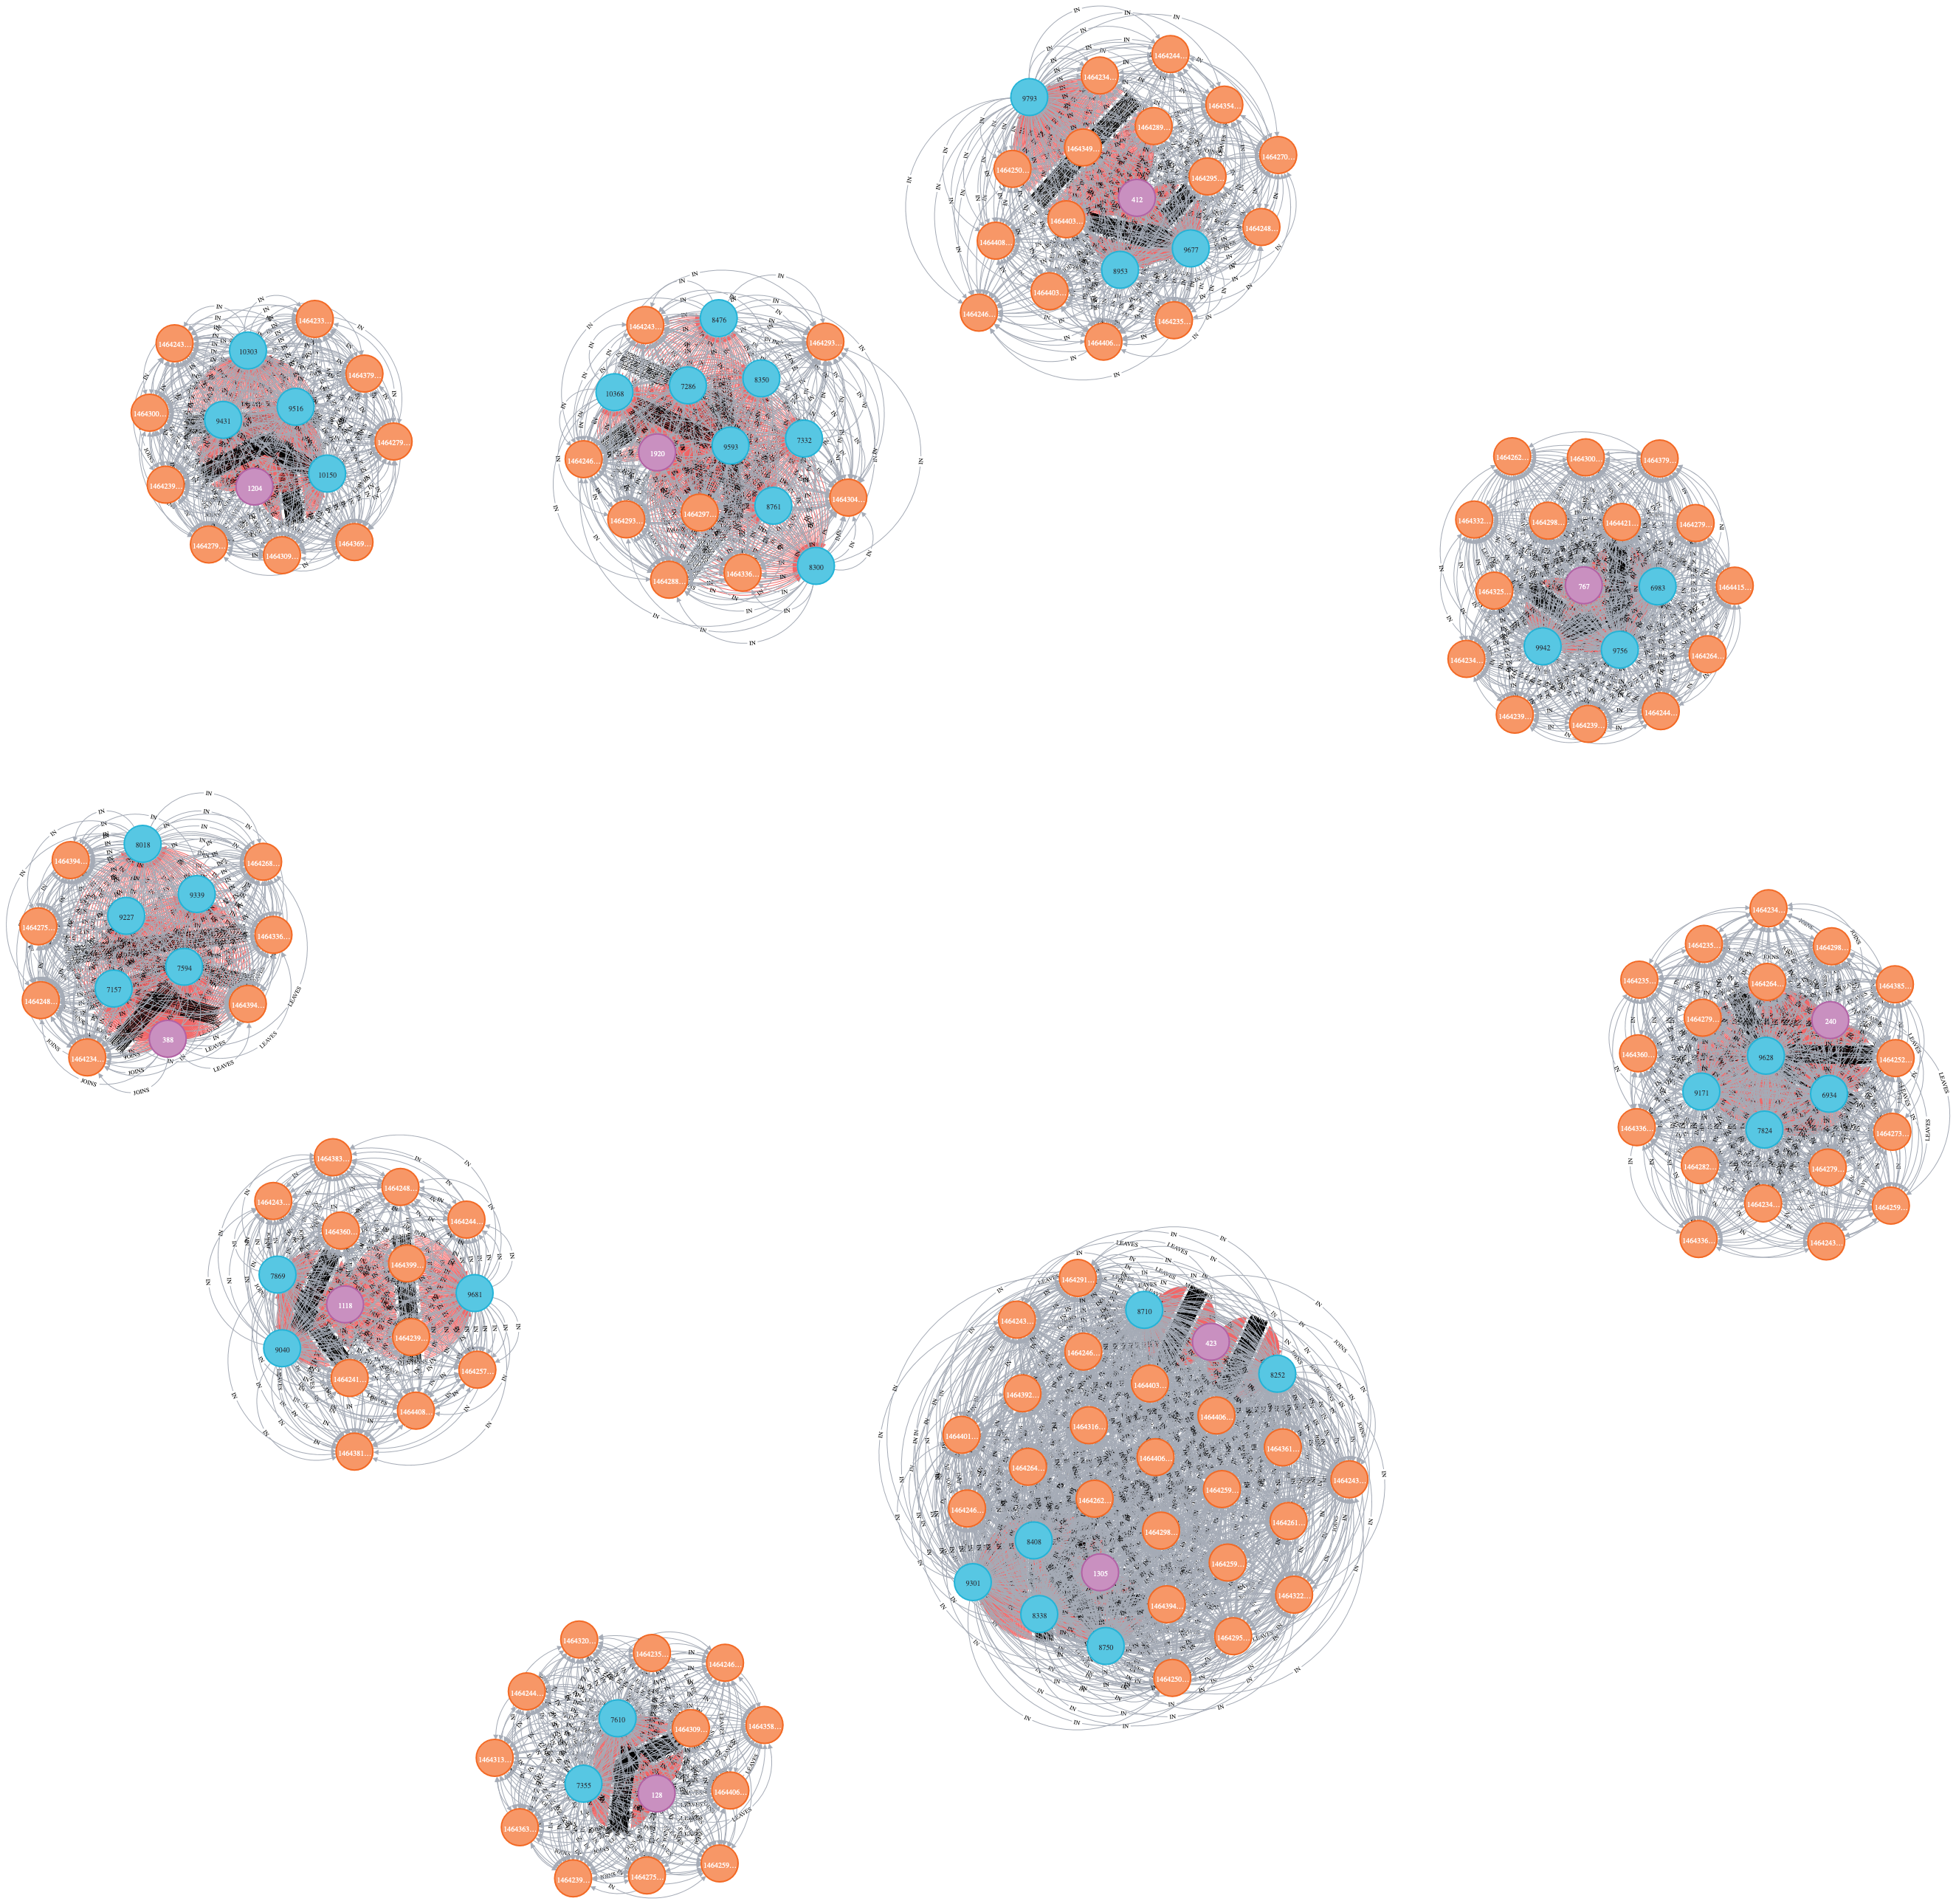
\includegraphics[scale=0.15]{img/Neo4j/graph1-filter.png}
    \centering
    \caption{Cypher filter 2}
    \label{fig:Graph 2 filtered}
  \end{figure}
\end{landscape}